\documentclass[10pt]{article}
\usepackage[a4paper,margin=1.6cm,top=1.3cm,bottom=1.3cm]{geometry}
\usepackage[T1]{fontenc}
\usepackage{lmodern}
\usepackage{microtype}
\usepackage{booktabs}
\usepackage{graphicx}
\usepackage{enumitem}
\usepackage{xcolor}
\usepackage[colorlinks=true,linkcolor=black,citecolor=black,urlcolor=blue]{hyperref}
\setlist{nosep,leftmargin=1.2em,topsep=1pt}
\setlength{\parindent}{0pt}
\setlength{\parskip}{3pt}
\pagestyle{empty}
\newcommand{\head}[1]{\par\smallskip{\large\bfseries #1}\par}
\newcommand{\sect}[1]{\par\smallskip{\bfseries\color{black!80} #1}\par}

\begin{document}
\head{Idea 7 PoC --- The fourth-quarter earnings dip}
\textit{Proof of concept, October 2026. Code: \texttt{idea07\_q4\_dip/run.py}.}

\sect{Question and design}
US firms report fourth-quarter earnings far below the first three quarters (Kapons and Binz), largely because of
year-end write-downs and earnings management (Das, Shroff and Zhang, 2009). Do Chinese firms show a similar Q4 dip?
Do earnings forecasts and prices anticipate it? For 25{,}442 firm-years (FY2004--2019) with all four standalone
quarters, $DIP=(Q4-\overline{Q1..Q3})/\sigma$, where $\sigma$ is the SD of the firm's past SRW errors. The tests are:
(a) the size and persistence of the dip; (b) the mean scaled SRW and XGBoost forecast errors by fiscal quarter;
(c) the size-adjusted return in the annual-report month, regressed on the XGBoost surprise plus either last year's
dip (predictable) or the run-rate surprise that a naive extrapolator would perceive. Regressions have month fixed
effects, with SEs clustered by month.

\begin{center}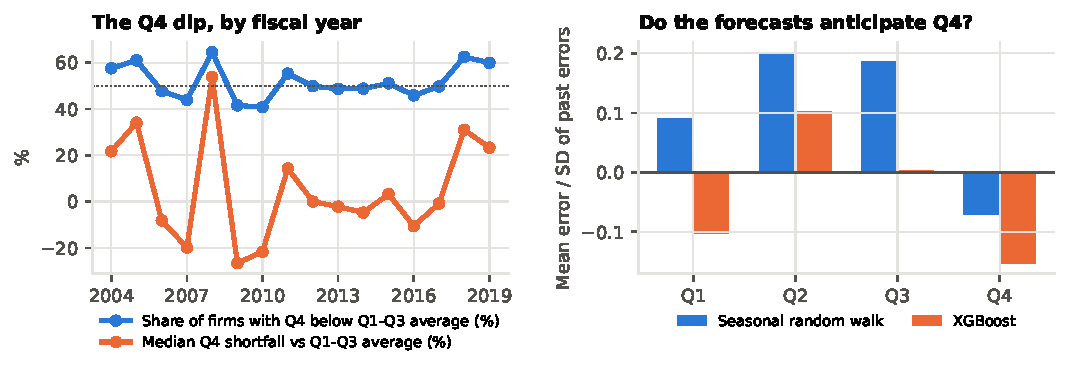
\includegraphics[width=0.97\textwidth]{results/fig_main.pdf}\end{center}

\begin{center}\small
\begin{tabular}{lcc}
\toprule
Annual-report month & Announcement month & Months $+1$ to $+3$\\
\midrule
$SUE^{XGB}$ & 0.41 (7.4) & 0.36 (3.1)\\
Last year's dip $DIP_{t-1}$ (known in advance) & 0.12 (4.9) & 0.00 (0.0)\\
\midrule
Run-rate surprise, replacing $DIP_{t-1}$ & 0.01 (0.2) & $-0.15$ ($-1.7$)\\
\bottomrule
\end{tabular}\\[2pt]
{\footnotesize \% return per unit ($t$). The SD of $DIP_{t-1}$ is 4.3, so one SD of past dip is worth about 0.5\% at the
annual report. Persistence of the dip: slope 0.17 ($t=4.2$).}
\end{center}

\sect{Findings}
\begin{itemize}
\item \textbf{No structural Q4 dip in China, but an event-driven one.} In normal years about half of firms report
  Q4 below their Q1--Q3 average. Large dips cluster in bad years: 2004--05, 2008, and 2018--19, the goodwill-impairment
  wave, when the median Q4 fell 31\% short. They also cluster in loss-making firms (mean $DIP$ $-0.71$ against
  $-0.25$), consistent with year-end big baths rather than a calendar effect.
\item \textbf{The statistical forecasts are not biased for Q4.} Mean scaled errors in Q4 are small and insignificant
  for both the SRW ($t=-0.4$) and XGBoost ($t=-0.6$). The time-series models have no systematic Q4 problem to
  correct.
\item \textbf{Prices under-anticipate habitual dippers.} Holding the XGBoost surprise fixed, firms with a large dip
  last year earn lower returns in the annual-report month (about 0.5\% per SD), with no reversal afterwards.
  Investors do not behave like naive run-rate extrapolators: the run-rate surprise adds nothing.
\end{itemize}

\sect{Assessment and next steps}
The original hypothesis, a predictable seasonal bias in forecasts, is not supported on these data. The surviving
result is narrower: a persistent, firm-specific year-end shortfall that prices do not fully anticipate. Without an
analyst FY forecast, the central ``do analysts anticipate the dip?'' test cannot be run. It needs I/B/E/S FY1
consensus at the Q3 report. A more promising reframing is the 2018 goodwill-impairment wave as a big-bath event
study. Overall this idea ranks lowest of Section B.
\end{document}
